\section{Galactic Lensing Diagnostic Plan}\label{manual:galactic-lensing-diagnostic-plan}
\aodnoteblock{Scope}{This section applies the current A\(\Omega\)D field-ring and \(\delta_3\) notation to a staged galactic-lensing diagnostic plan. It is a manual/application plan with an explicit L3 data-package gate.}
\aodprovenance{main:subsec:fractal-field-ring-gate; main:sec:field-dynamics; manual \secref{manual:cross-return-short-window}; manual \secref{manual:prediction-test-registry}.}
\aodliteraturenote{SWELLS target lane: Treu et al.~\cite{treu-swells-2011}, Brewer et al.~\cite{brewer-swells-2012}.}

\subsection{Lensing lanes}\label{manual:lensing-status-lock}
\small
\begin{longtable}{p{0.24\textwidth}p{0.10\textwidth}p{0.56\textwidth}}
\caption{Galactic lensing data and projection lanes.}\label{tab:manual-lensing-status-lock}\\
\toprule
Lane & Class & Active fields\\
\midrule
\endfirsthead
\toprule
Lane & Class & Active fields\\
\midrule
\endhead
Toy 1 & L0 & exact internal \(\delta_3\) fixture\\
SPARC5 & L1 & radial lens-medium data-support class; lens target fields are carried by SWELLS or L3 rows\\
SWELLS K0 & L2 & target acquisition\\
SWELLS K1 & L1/L2 & retained baseline\\
SWELLS K2/K3 & L1/L2 & audit diagnostics\\
K4 & L3 & higher-resolution lensing input-manifest row\\
L3 lensing input package & L3 & L3 input-manifest row; required fields: independent 3D medium fields, time-flow inputs, radiation-current gates, target-side quarantine, null controls, and audit\\
\bottomrule
\end{longtable}
\normalsize

\subsection{Field-ring spine}\label{manual:lensing-field-ring-spine}
The lensing fixture uses a discrete exoshedding field-ring calculation. The value table records the evaluated gate values.
\[
B_{\mathrm{lens}}=(\partial_TF_{\mathrm{exo}},\omega_{\mathrm{lens}}).
\]
\[
T^0_k=\sum_i S^{(i)}_k.
\]
\[
T^\times_k
=
T^0_k+
\sum_{(i,j)\in E_{\mathrm{return}}}C^\times_{ij,k}(B_{\mathrm{lens}}).
\]
\[
T^\times_k-T^0_k
=
\sum_{(i,j)\in E_{\mathrm{return}}}C^\times_{ij,k}(B_{\mathrm{lens}}).
\]
\[
\Delta^{\mathbb Z}_k=T^\times_k-O_k,
\qquad
\delta_{3,k}(T^\times,O)=(s^{(3)}_k,m_k),
\qquad
m_k=|\Delta^{\mathbb Z}_k|.
\]
\[
\delta_3(T^\times,O)=(\delta_{3,k})_{k\in K}.
\]
\begin{figure}[H]
\centering
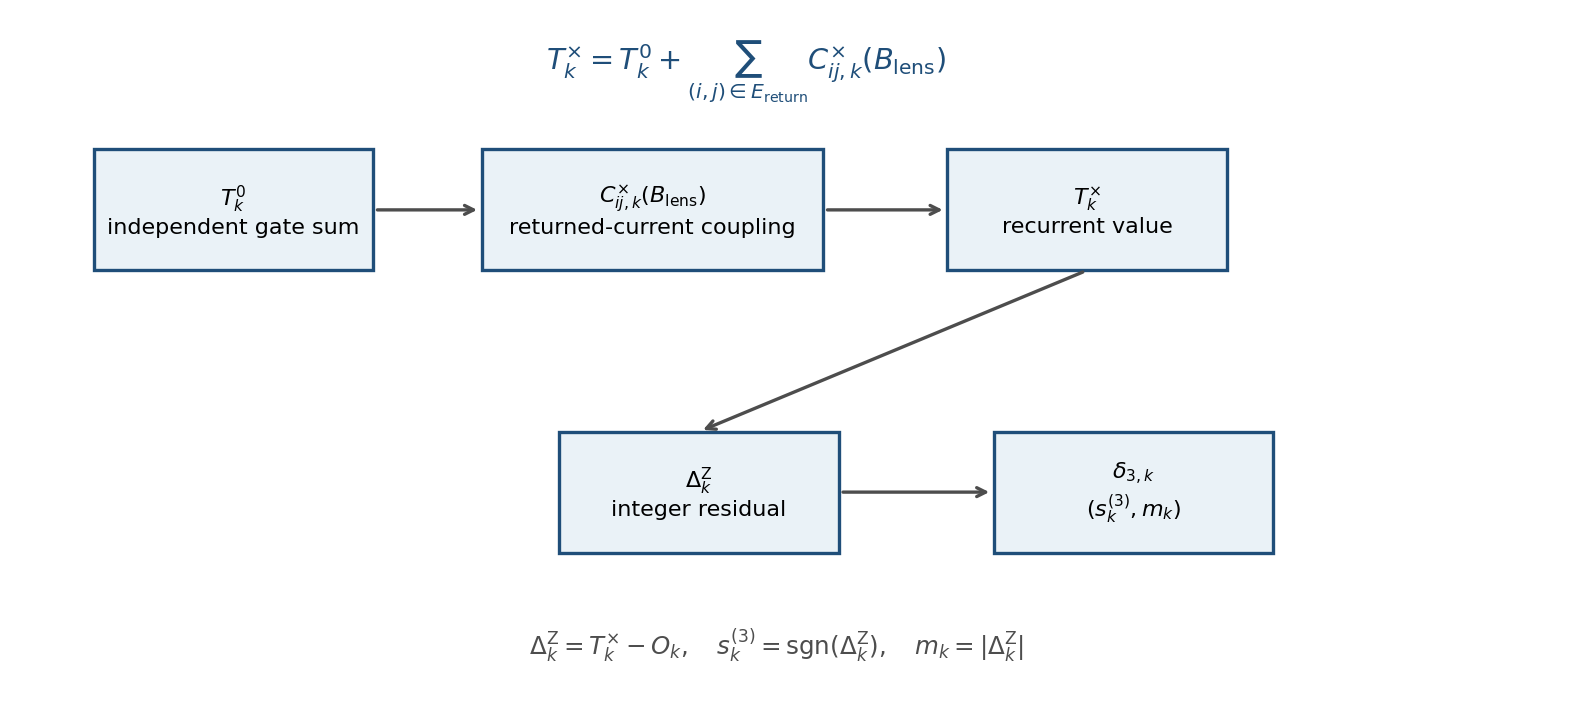
\includegraphics[width=0.86\linewidth]{figures/lensing/02_frg_value_identity_delta3.png}
\caption{FRG value identity and \(\delta_3\) audit. Gate values \(T^0\), \(C^\times\), and \(T^\times\) are computed before the fixture comparator joins.}
\label{fig:manual-lensing-frg-delta3}
\end{figure}

\subsection{Toy fixture lane}\label{manual:lensing-toy-fixture-lane}
Toy 1 is the exact internal lensing toy. It belongs to the manual fixture lane and registry.
\small
\begin{longtable}{p{0.36\textwidth}r}
\caption{Toy 1 exact internal \(\delta_3\) fixture summary.}\label{tab:manual-lensing-toy-summary}\\
\toprule
Quantity & Value\\
\midrule
\endfirsthead
\toprule
Quantity & Value\\
\midrule
\endhead
gates & 16\\
target bins & 13\\
events & 18\\
caustic bins & 0, 2\\
\(\delta_3\) total \(m\) & 0\\
checks passed & 11/11\\
\bottomrule
\end{longtable}
\normalsize
\begin{figure}[H]
\centering
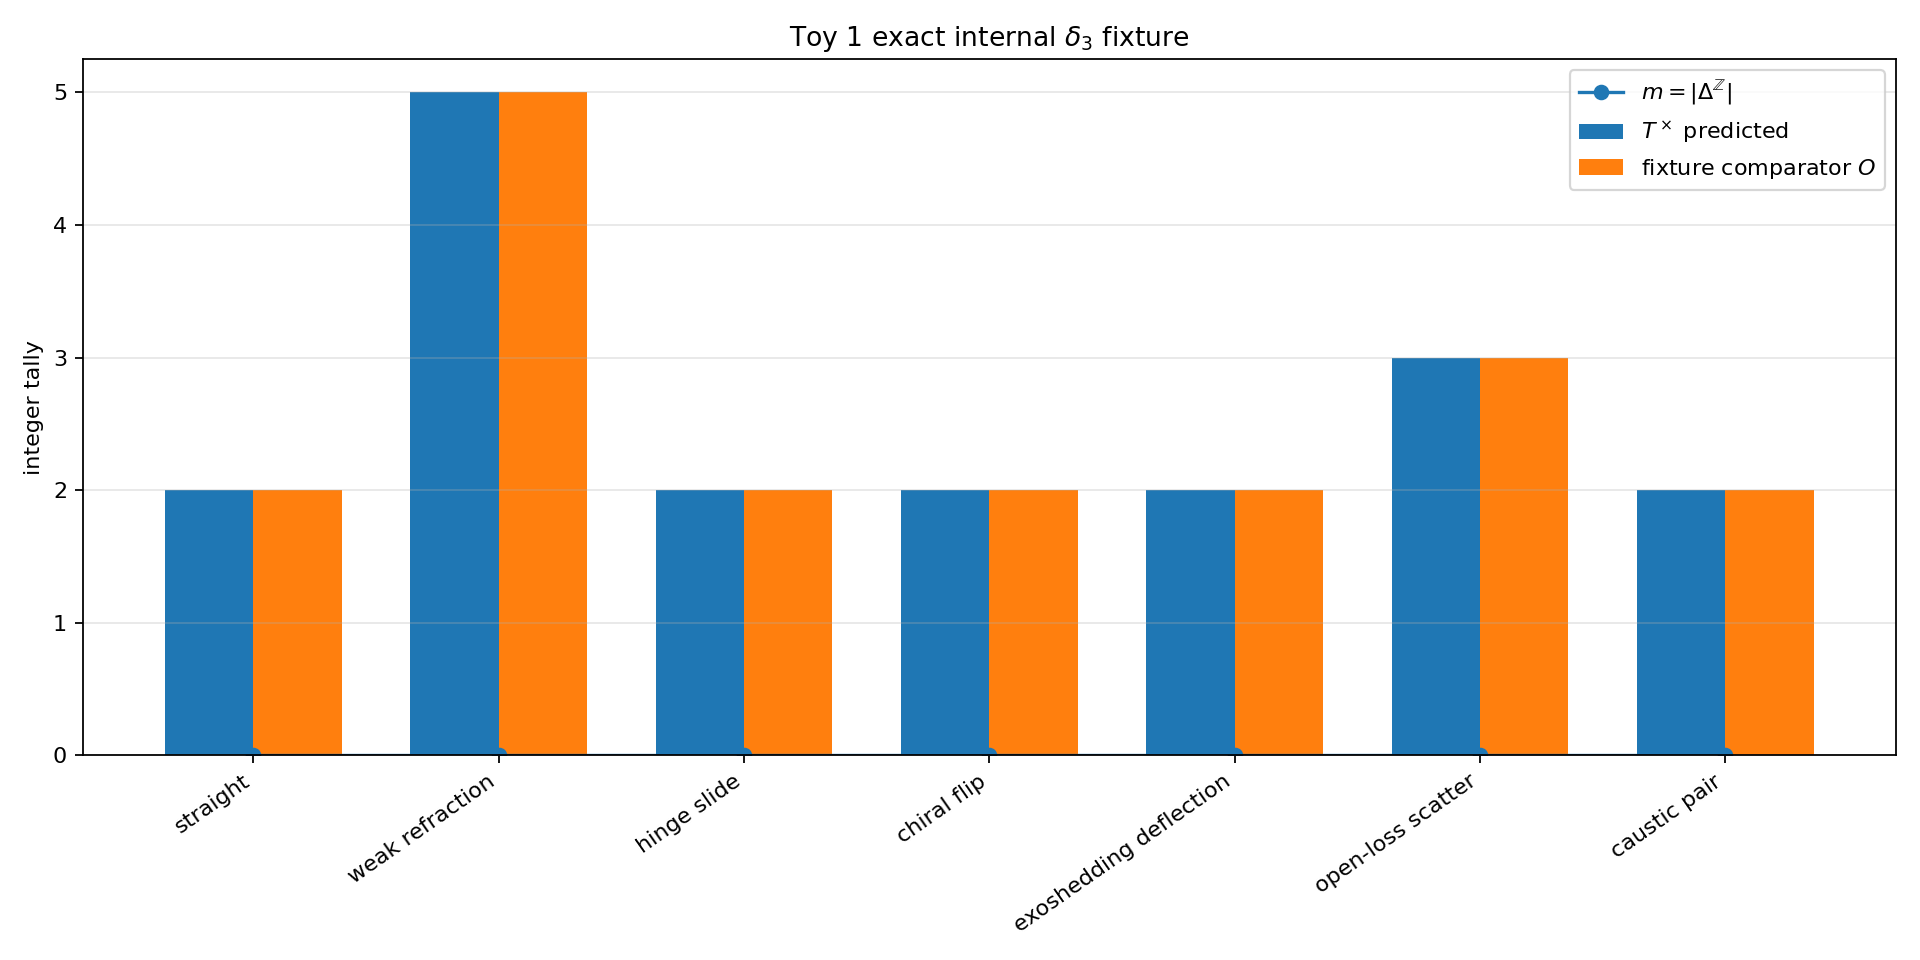
\includegraphics[width=0.86\linewidth]{figures/lensing/01_toy1_delta3_class_tallies.png}
\caption{Toy 1 exact internal \(\delta_3\) class tallies.}
\label{fig:manual-lensing-toy-delta3}
\end{figure}

\subsection{SPARC5 lens-medium 2D data fixture}\label{manual:lensing-sparc5-medium-diagnostic}
SPARC5 instantiates a radial lens-medium data-support class. It supplies radial field-medium inputs for declared projection/readout runs. Image-count, Einstein-radius, image-position, and shear target fields are target-side quantities carried by SWELLS or an L3 input package.
\scriptsize
\begin{longtable}{p{0.10\textwidth}p{0.05\textwidth}p{0.05\textwidth}p{0.06\textwidth}p{0.06\textwidth}p{0.10\textwidth}p{0.09\textwidth}p{0.18\textwidth}p{0.15\textwidth}}
\caption{SPARC5 lens-medium summary.}\label{tab:manual-lensing-sparc5-summary}\\
\toprule
Galaxy & Bins & Gates & Events & Caustic & Median $|\Delta A_\gamma|$ & Max $|\Delta A_\gamma|$ & Dominant class & Status\\
\midrule
\endfirsthead
\toprule
Galaxy & Bins & Gates & Events & Caustic & Median $|\Delta A_\gamma|$ & Max $|\Delta A_\gamma|$ & Dominant class & Status\\
\midrule
\endhead
NGC2403 & 73 & 32 & 44 & 12 & 1.1667 & 1.9 & exoshedding deflection & lens-medium\\
NGC3198 & 43 & 32 & 44 & 12 & 1.2721 & 2.0 & exoshedding deflection & lens-medium\\
NGC6503 & 31 & 32 & 44 & 12 & 1.3801 & 2.4706 & exoshedding deflection & lens-medium\\
NGC2841 & 50 & 32 & 41 & 9 & 1.2416 & 1.7647 & exoshedding deflection & lens-medium\\
DDO154 & 12 & 32 & 46 & 14 & 1.2941 & 2.625 & exoshedding deflection & lens-medium\\
\bottomrule
\end{longtable}
\normalsize

\begin{figure}[H]
\centering
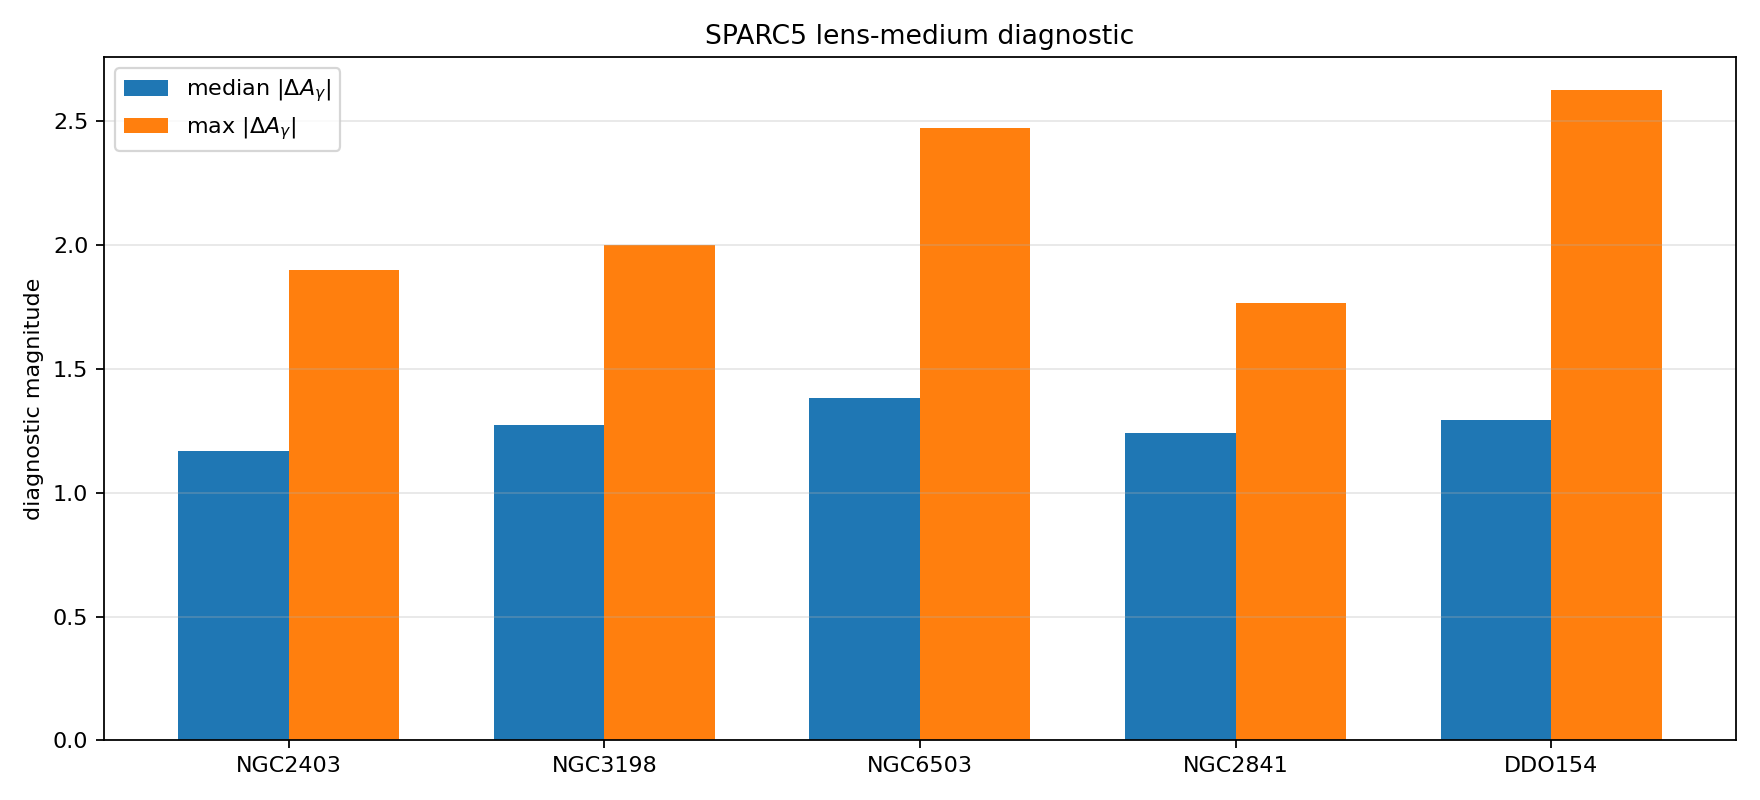
\includegraphics[width=0.82\linewidth]{figures/lensing/03_sparc5_lens_medium_phase_proxy.png}
\caption{SPARC5 radial lens-medium data-support class. The plotted quantities are 2D medium-proxy coordinates; lensing targets are carried by SWELLS or a higher-resolution class.}
\label{fig:manual-lensing-sparc5-proxy}
\end{figure}
\begin{figure}[H]
\centering
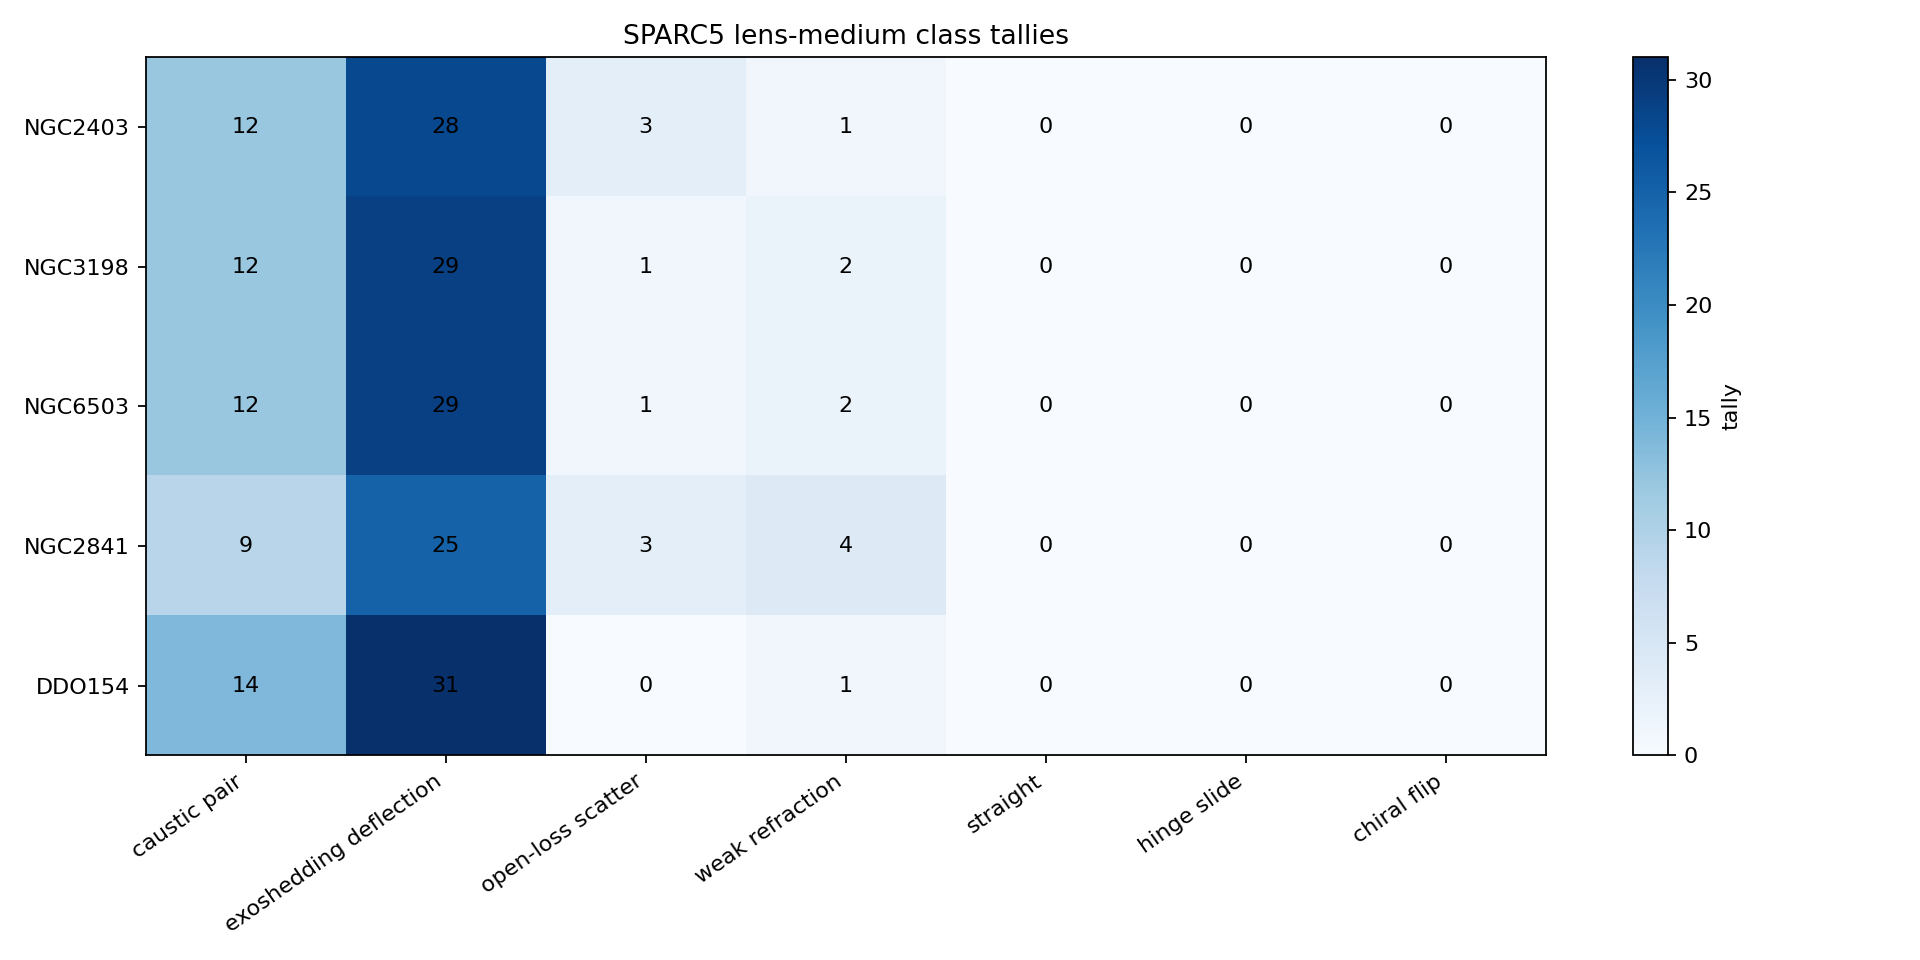
\includegraphics[width=0.82\linewidth]{figures/lensing/04_sparc5_class_tally_heatmap.png}
\caption{SPARC5 lens-medium class tallies. The dominant declared route class is recorded for audit.}
\label{fig:manual-lensing-sparc5-classes}
\end{figure}

\subsection{SWELLS target lane}\label{manual:lensing-swells-lane}
SWELLS supplies target-side acquisition fields for the lensing lane.
\scriptsize
\begin{longtable}{p{0.34\textwidth}p{0.34\textwidth}p{0.16\textwidth}}
\caption{SWELLS K0 target-side acquisition fields.}\label{tab:manual-lensing-swells-k0}\\
\toprule
Target family & Class $k$ & $O$ tally\\
\midrule
\endfirsthead
\toprule
Target family & Class $k$ & $O$ tally\\
\midrule
\endhead
strong-lens presence & modelled lens & 20\\
grade & A & 19\\
grade & B & 1\\
Einstein radius bin & \(\theta_E<0.75\) & 3\\
Einstein radius bin & \(0.75\le\theta_E<1.00\) & 9\\
Einstein radius bin & \(\theta_E\ge1.00\) & 8\\
\(\sigma_{\mathrm{SIE}}\) bin & \(\sigma<200\) & 8\\
\(\sigma_{\mathrm{SIE}}\) bin & \(200\le\sigma<230\) & 7\\
\(\sigma_{\mathrm{SIE}}\) bin & \(\sigma\ge230\) & 5\\
\bottomrule
\end{longtable}
\normalsize

\scriptsize
\begin{longtable}{p{0.05\textwidth}p{0.24\textwidth}p{0.09\textwidth}p{0.10\textwidth}p{0.09\textwidth}p{0.15\textwidth}p{0.22\textwidth}}
\caption{SWELLS K1/K2/K3 diagnostic comparison.}\label{tab:manual-lensing-swells-k123}\\
\toprule
Run & Input basis & $\theta_E$ $\delta_3$ $m_{\rm tot}$ & $\theta_E$ match [\%] & $\sigma$ $\delta_3$ $m_{\rm tot}$ & Decision & Reason\\
\midrule
\endfirsthead
\toprule
Run & Input basis & $\theta_E$ $\delta_3$ $m_{\rm tot}$ & $\theta_E$ match [\%] & $\sigma$ $\delta_3$ $m_{\rm tot}$ & Decision & Reason\\
\midrule
\endhead
K1 & \(\sigma_{\mathrm{SDSS}}\) + H\(\alpha\) + axis ratio & 8 & 40.0 & 4 & retained baseline & lowest retained $\delta_3$ residual\\
K2 & K1 + redshift geometry context & 18 & 40.0 & 4 & audit diagnostic record & over-amplified high \(\theta_E\) class\\
K3 & Paper I Table 2 bulge/disk medium fields & 10 & 33.3333 & 12 & audit diagnostic record & under-resolved observable map with current medium data\\
\bottomrule
\end{longtable}
\normalsize

K1 is retained as the baseline. K2 and K3 are audit diagnostics.
\begin{figure}[H]
\centering
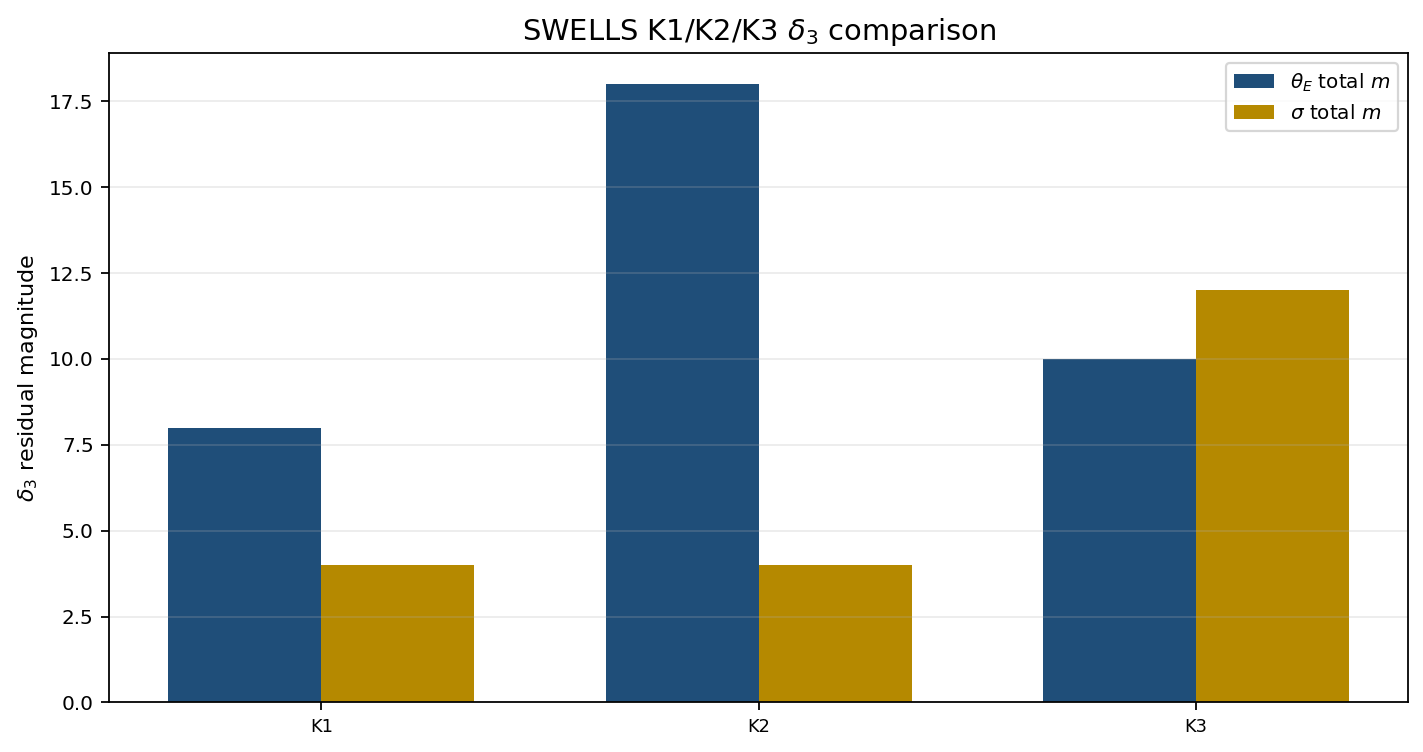
\includegraphics[width=0.82\linewidth]{figures/lensing/05_swells_k_comparison_delta3.png}
\caption{SWELLS K1/K2/K3 \(\delta_3\) comparison. K2/K3 are audit diagnostics with \(\delta_3\) comparison tallies.}
\label{fig:manual-lensing-swells-comparison}
\end{figure}
\begin{figure}[H]
\centering
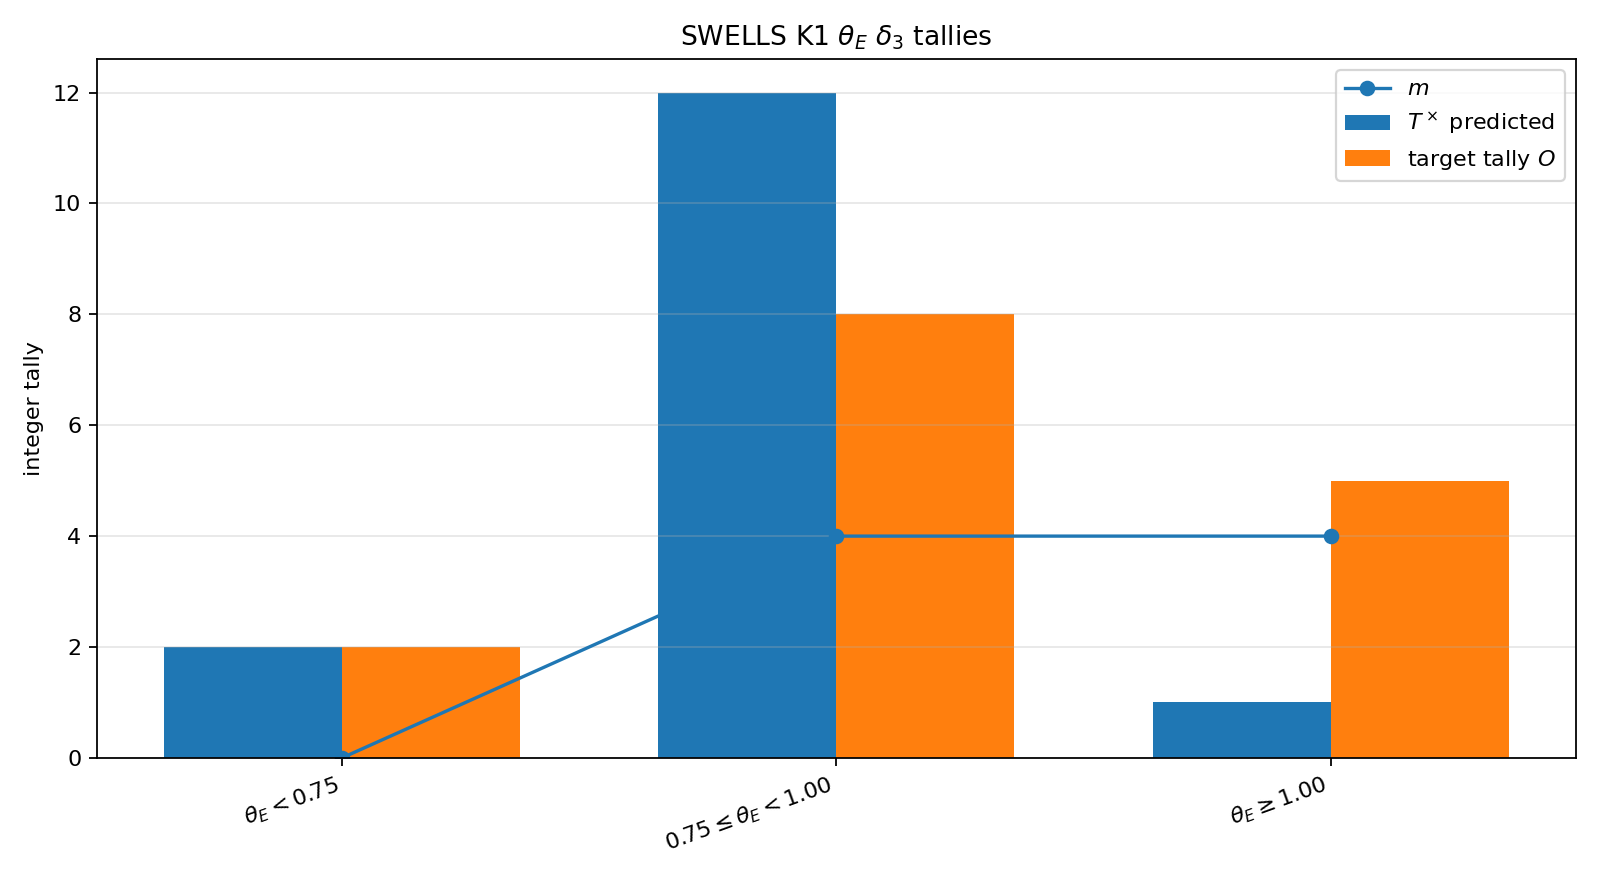
\includegraphics[width=0.82\linewidth]{figures/lensing/06_swells_k1_thetaE_delta3_tallies.png}
\caption{SWELLS K1 retained-baseline \(\theta_E\) \(\delta_3\) tallies.}
\label{fig:manual-lensing-swells-k1}
\end{figure}

\subsection{K4 input gate}\label{manual:lensing-k4-input-gate}
K4 is the higher-resolution lensing input-manifest row for independent 3D and time-flow inputs.
\scriptsize
\begin{longtable}{p{0.18\textwidth}p{0.35\textwidth}p{0.22\textwidth}p{0.16\textwidth}}
\caption{K4 independent 3D + time-flow input gate.}\label{tab:manual-lensing-k4-gate}\\
\toprule
Input group & Required field & Source status & Gate\\
\midrule
\endfirsthead
\toprule
Input group & Required field & Source status & Gate\\
\midrule
\endhead
3D density fields & stellar density \(\rho_\star(R,z,\theta)\) & external / 3D proxy & required\\
3D density fields & gas density \(\rho_{\mathrm{gas}}(R,z,\theta)\) & external / 3D proxy & required\\
velocity and flow fields & gas and stellar velocity vector field & IFU / H I / H\(\alpha\) & required\\
velocity and flow fields & line-of-sight flow and bobbing/slosh phase & time / kinematic proxy & required\\
momentum fields & angular momentum and radial/linear momentum & independent kinematics & required\\
time-window state & duration/cadence windows for flow transfer & declared pre-score & required\\
lensing target side & image-position bins & quarantined target & required\\
lensing target side & Einstein-radius bins and image count classes & quarantined target & required\\
audit controls & null / permutation controls & declared pre-score & required\\
\bottomrule
\end{longtable}
\normalsize

\begin{figure}[H]
\centering
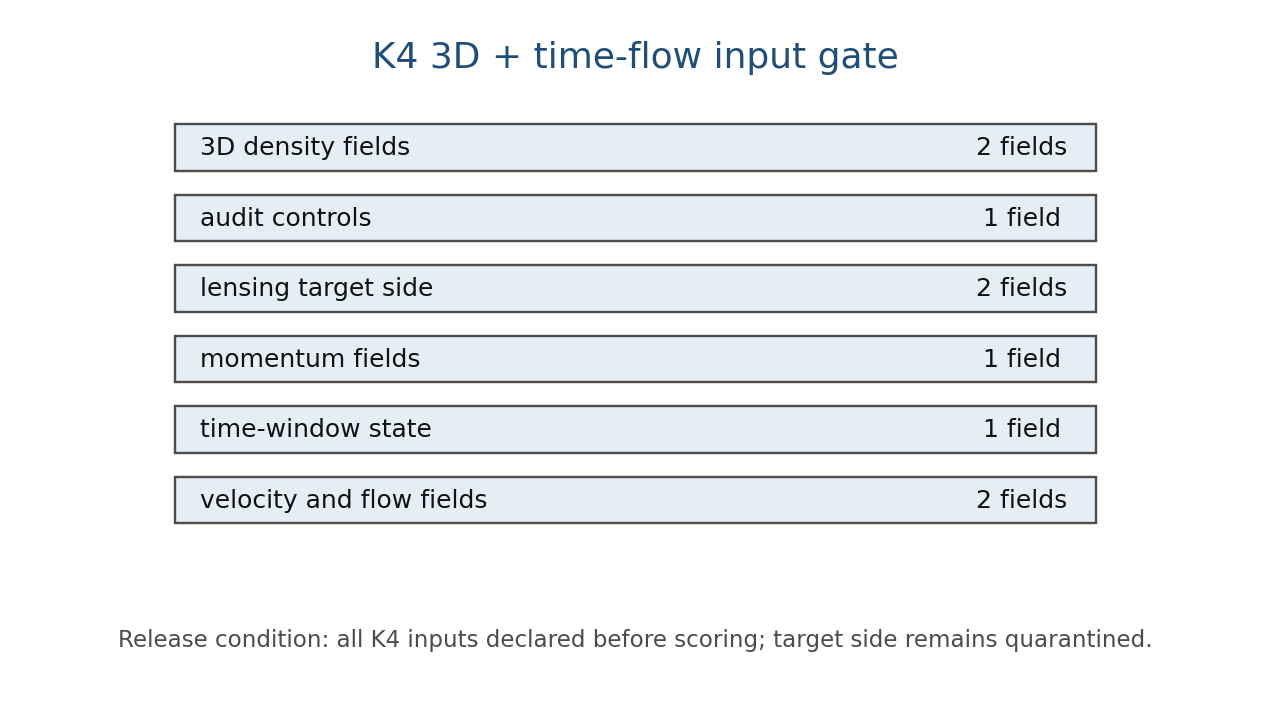
\includegraphics[width=0.86\linewidth]{figures/lensing/07_k4_3d_timeflow_input_gate.png}
\caption{K4 higher-resolution lensing data-support gate. The L3 input package records independent 3D + time-flow medium data before the target side joins.}
\label{fig:manual-lensing-k4-gate}
\end{figure}

\subsection{Target-side quarantine and release gate}\label{manual:lensing-release-gate}
The A\(\Omega\) input side carries medium fields, gate values, and declared prediction values. The target side carries image-position, Einstein-radius, and image-count targets after prediction values freeze.
\begin{figure}[H]
\centering
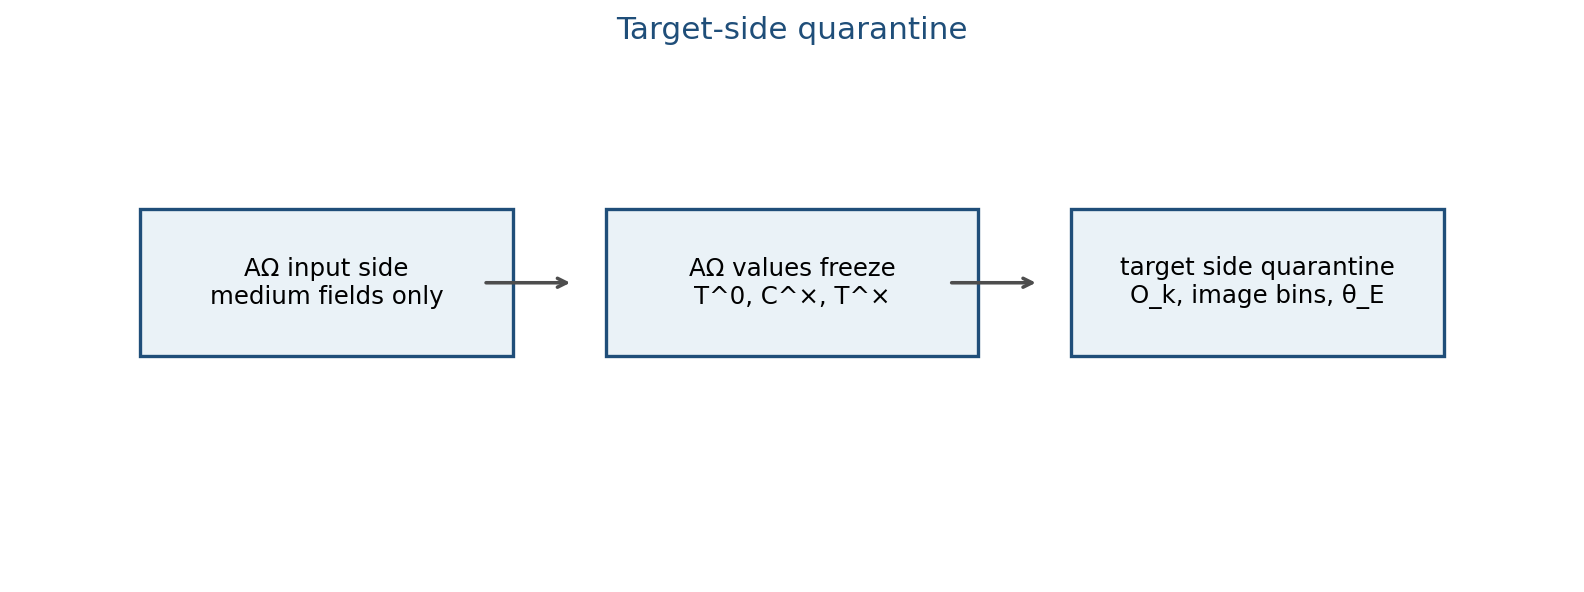
\includegraphics[width=0.86\linewidth]{figures/lensing/08_target_quarantine.png}
\caption{Target-side quarantine. A\(\Omega\) values freeze before target tallies join.}
\label{fig:manual-lensing-target-quarantine}
\end{figure}
\begin{figure}[H]
\centering
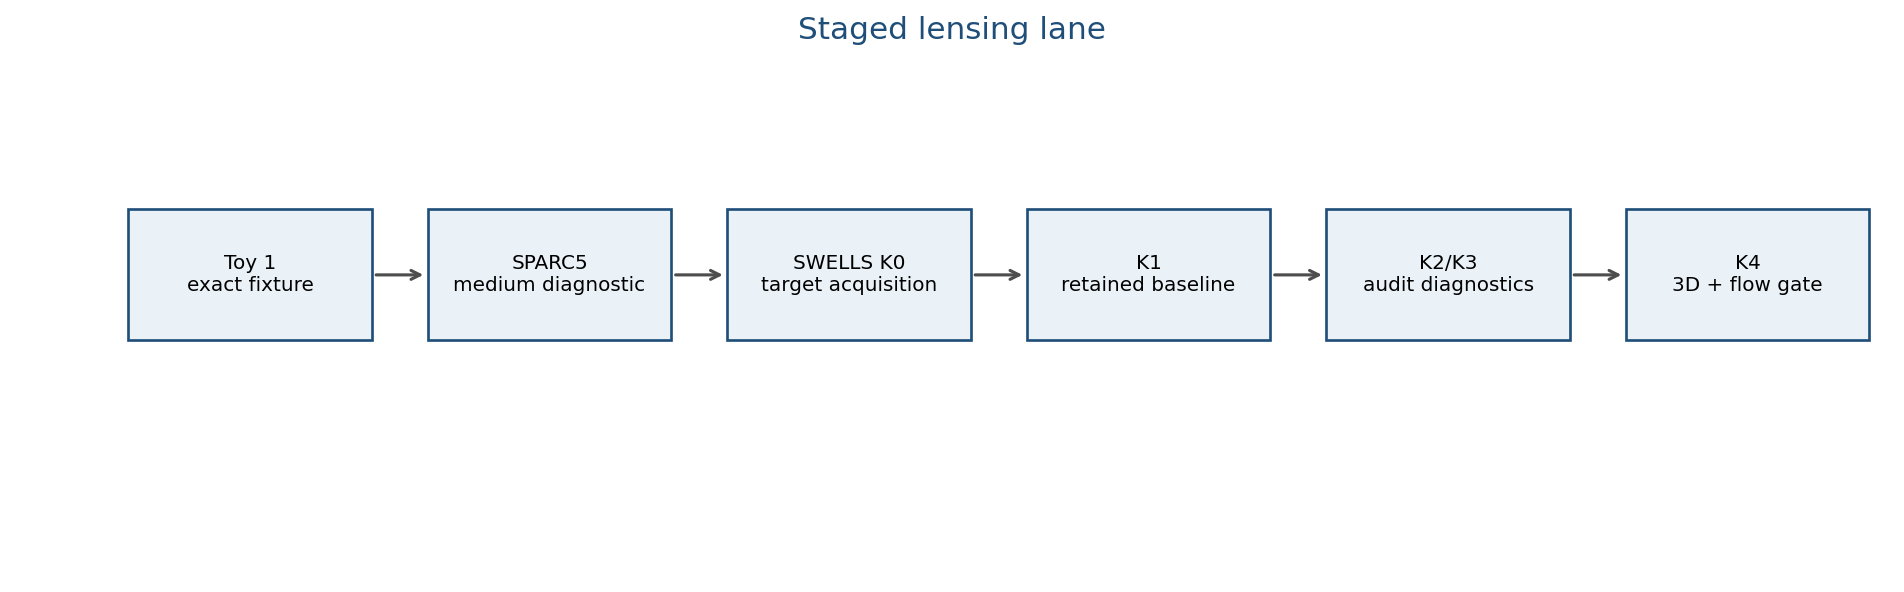
\includegraphics[width=0.90\linewidth]{figures/lensing/09_staged_lensing_lane.png}
\caption{Staged galactic lensing lane. Toy fixtures, the SPARC5 2D data fixture, SWELLS acquisition, retained baseline, K2/K3 audit outputs, and K4 gate are kept distinct.}
\label{fig:manual-lensing-staged-lane}
\end{figure}
\begin{figure}[H]
\centering
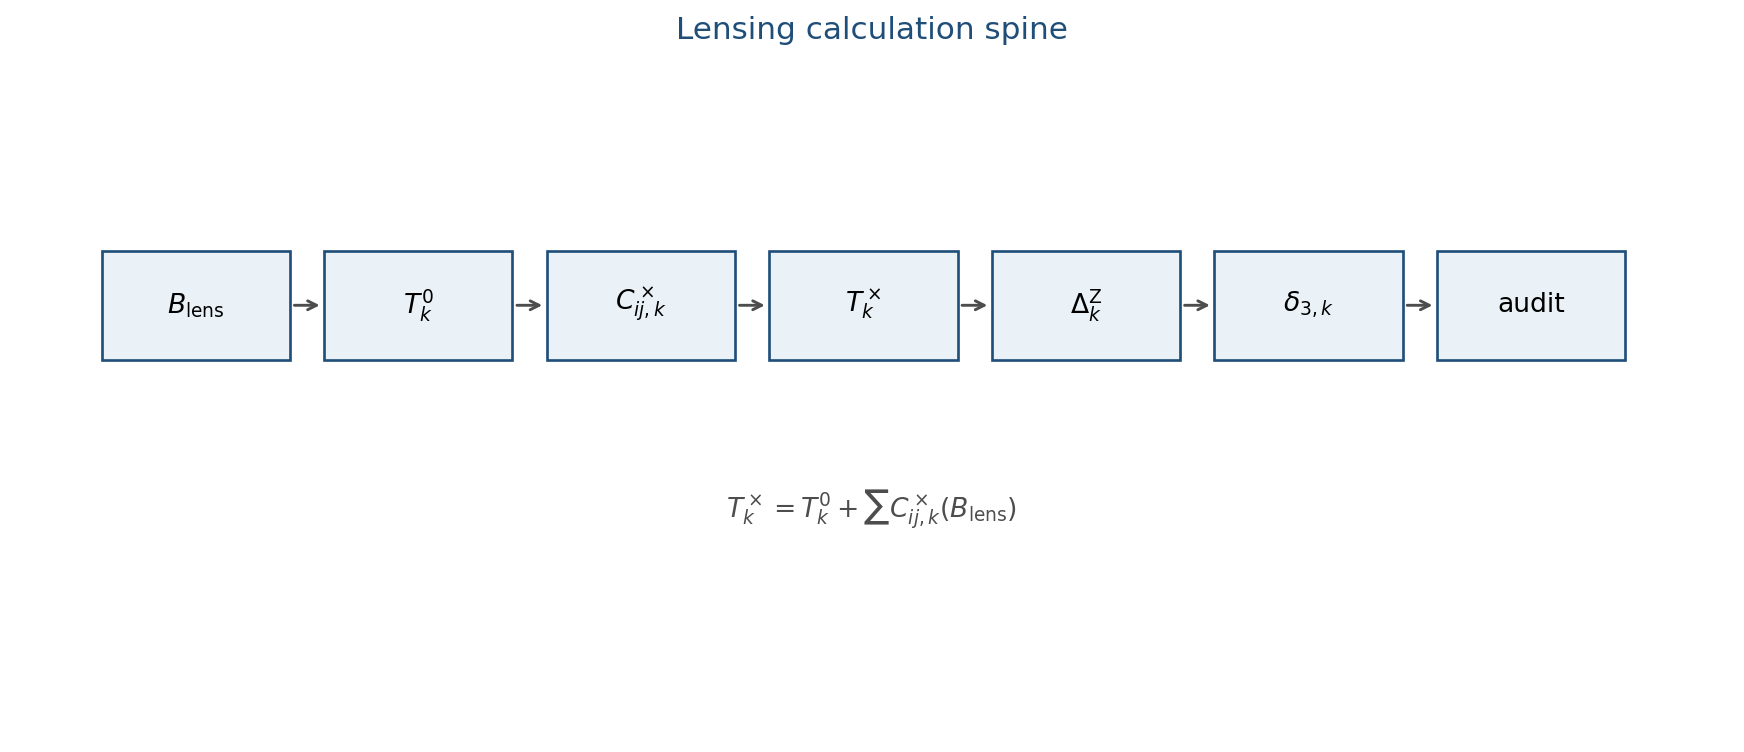
\includegraphics[width=0.90\linewidth]{figures/lensing/10_lensing_calculation_spine.png}
\caption{Galactic lensing calculation spine. The \(U\)-projection and lensing targets remain downstream of declared field-ring values.}
\label{fig:manual-lensing-calculation-spine}
\end{figure}

A completed L3 lensing record carries declared medium fields, declared radiation-current gates, declared target-side quarantine, computed \(T^0\), \(C^\times\), and \(T^\times\), declared \(\lambda_{\mathrm{lens}}\), \(\delta_3\) residual table, null controls, audit, and lens residuals after A\(\Omega\) values freeze.
